\section{Simulation}
To test some \ac{cpp} algorithms is worth to implement an environment which allows to drive a drone autonomously in a safe way, without any risk of collision. PX4 offers different simulators which allow to develop \ac{sitl} simulation \cite{px4_simulation}. More in details, in the section named \textit{MAVROS Offboard control example (Python)} \cite{px4_ros_mavros} there is a useful example on how to setup PX4, Gazebo and MAVROS to run a simulation.

To implement a complete pipeline which allows to develop \ac{cpp} algorithms, simulate the quadcopter and analyse the result MATLAB has been employed beside the simulator structure which exploit PX4, Gazebo and MAVROS, mentioned above. MATLAB is used to determine the area, develop the \ac{cpp} algorithms and pass the waypoint to the simulator. After the simulation phase, which is executed in Gazebo environment the results are visualized and analysed in MATLAB again.

MATLAB is executed in Windows environment, while PX4 software stack, Gazebo and of course \ac{ros} are executed in \ac{wsl} environment (more specifically in Ubuntu 20.04).

\subsection{MATLAB code} 
There are two main files called \texttt{main.m} and \texttt{WSL\_connection.m}; the first one deals with the definition of the target area by the user, the execution of the \ac{cpp} algorithm and consequently the determination of waypoints in space. The second one is devoted to establish the connection with \ac{wsl} to send the waypoint calculated in the \texttt{main.m} file.
\subsubsection*{Main.m code}
As mentioned previously the \texttt{main.m} code is responsible for determining the area of interest and the waypoint calculation.
The first section allows the user to select an area by specifying the latitude and longitude as shown in \ref{fig:target_area_selection}. After the selection procedure the area is converted in local coordinate expressed in meters. This further step is needed because waypoints will be calculated based on robot's footprint.
\lstinputlisting[language=Octave, linerange={5-34}, firstnumber=5]{../simulator/main.m}
\begin{figure}[hbt!]
	\centering
	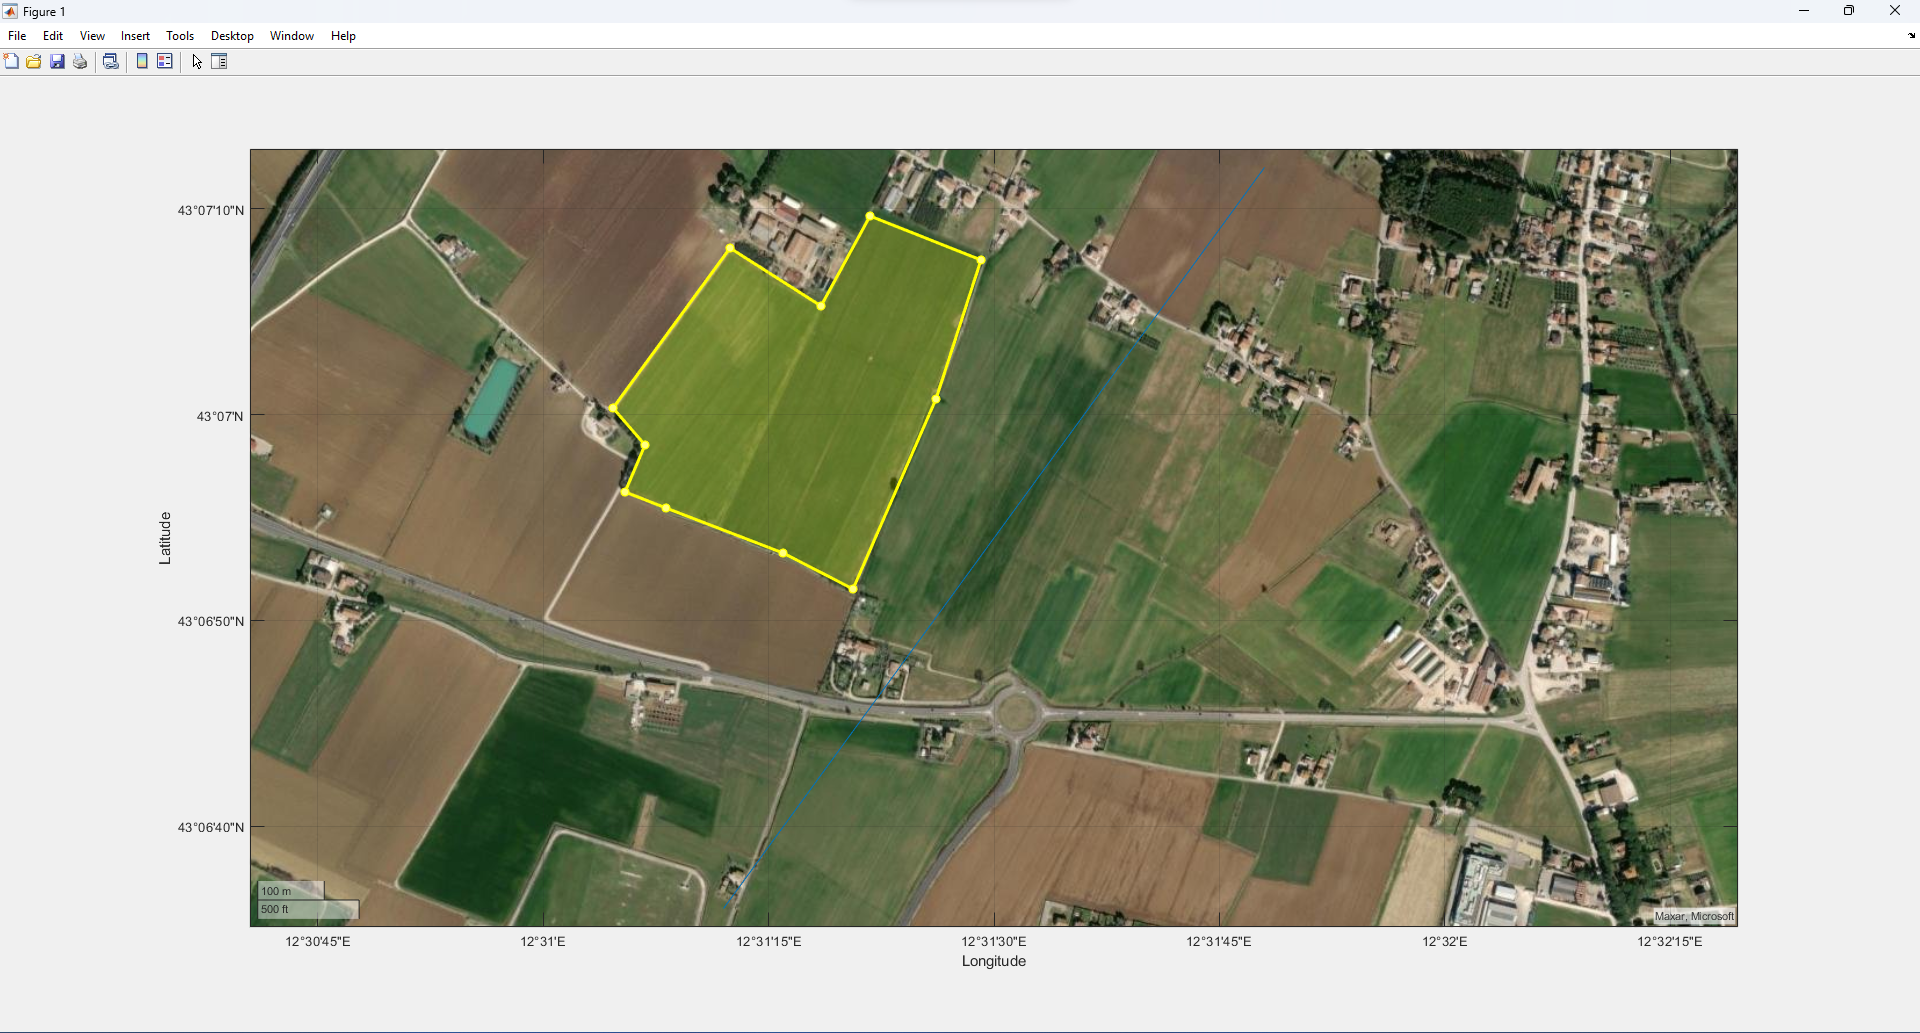
\includegraphics[width=\linewidth]{images/target_area_selection}
	\caption{Target area selection.}
	\label{fig:target_area_selection}
\end{figure}

The next section is devoted to the application of the \ac{cpp} algorithm to the selected area, it returns a 2D or 3D waypoints, these last ones will be passed to the simulator through the \texttt{WSL\_connection.m} file.
\lstinputlisting[language=Octave, linerange={39-74}, firstnumber=39]{../simulator/main.m}

\subsection{WSL\_connection.m code}
This script is responsible for the connection with \ac{wsl}, which means that allows MATLAB to interact with the rostopic executed on \ac{wsl}, it automatically recovers the ip addresses needed
\footnote{This code is tested in Windows system, to recover the addresses through Windows terminal and ubuntu shell type the following commands: 
\begin{itemize}
	\item In Ubuntu shell type \texttt{\$ ifconfig} and look for the address named \texttt{iner} under \texttt{eth0}. This is the variable named \texttt{ipAdd\_wsl}.
	\item In Windows terminal type \texttt{\$ ip config} and look for \texttt{IPv4 address} under \texttt{Ethernet Card vEthernet (WSL). This is the variable named \texttt{ipAdd\_Windows}}.
\end{itemize}}.
\lstinputlisting[language=Octave, linerange={1-23}, firstnumber=1]{../simulator/WSL_connection.m}

In addition, the second section is responsible of instantiating a new node which publish the waypoint list\footnote{The code assumes that there is a matrix variable named \texttt{waypoint3D}, wtih dimensions $N \times 3$, where $N$ represents the number of waypoint and the columns are the $xyz$ coordinates in the space.} in the topic named \texttt{/MATLAB\_waypoint}.
\lstinputlisting[language=Octave, linerange={26-47}, firstnumber=26]{../simulator/WSL_connection.m}
